\pdfminorversion=4
\documentclass[aspectratio=169]{beamer}

\mode<presentation>
{
  \usetheme{default}
  \usecolortheme{default}
  \usefonttheme{default}
  \setbeamertemplate{navigation symbols}{}
  \setbeamertemplate{caption}[numbered]
  \setbeamertemplate{footline}[frame number]  % or "page number"
  \setbeamercolor{frametitle}{fg=white}
  \setbeamercolor{footline}{fg=black}
} 

\usepackage[english]{babel}
\usepackage[utf8x]{inputenc}
\usepackage{tikz}
\usepackage{courier}
\usepackage{array}
\usepackage{bold-extra}
\usepackage{minted}
\usepackage[thicklines]{cancel}
\usepackage{fancyvrb}

\xdefinecolor{dianablue}{rgb}{0.18,0.24,0.31}
\xdefinecolor{darkblue}{rgb}{0.1,0.1,0.7}
\xdefinecolor{darkgreen}{rgb}{0,0.5,0}
\xdefinecolor{darkgrey}{rgb}{0.35,0.35,0.35}
\xdefinecolor{darkorange}{rgb}{0.8,0.5,0}
\xdefinecolor{darkred}{rgb}{0.7,0,0}
\definecolor{darkgreen}{rgb}{0,0.6,0}
\definecolor{mauve}{rgb}{0.58,0,0.82}

\title[2019-09-13-history-strangeloop]{The divergent histories of particle physics and computing}
\author{Jim Pivarski}
\institute{Princeton University -- IRIS-HEP}
\date{September 13, 2019}

\usetikzlibrary{shapes.callouts}

\begin{document}

\logo{\pgfputat{\pgfxy(0.11, 7.4)}{\pgfbox[right,base]{\tikz{\filldraw[fill=dianablue, draw=none] (0 cm, 0 cm) rectangle (50 cm, 1 cm);}\mbox{\hspace{-8 cm}
\includegraphics[height=1 cm]{princeton-logo-long.png}\hspace{0.1 cm}\raisebox{0.1 cm}{
\includegraphics[height=0.8 cm]{iris-hep-logo-long.png}}\hspace{0.1 cm}}}}}

\begin{frame}
  \titlepage
\end{frame}

\logo{\pgfputat{\pgfxy(0.11, 7.4)}{\pgfbox[right,base]{\tikz{\filldraw[fill=dianablue, draw=none] (0 cm, 0 cm) rectangle (50 cm, 1 cm);}\mbox{\hspace{-8 cm}
\includegraphics[height=1 cm]{princeton-logo.png}\hspace{0.1 cm}\raisebox{0.1 cm}{
\includegraphics[height=0.8 cm]{iris-hep-logo.png}}\hspace{0.1 cm}}}}}

% Uncomment these lines for an automatically generated outline.
%\begin{frame}{Outline}
%  \tableofcontents
%\end{frame}

% START START START START START START START START START START START START START

\begin{frame}{Prehistory}
\Large
\vspace{0.5 cm}
\begin{center}
We can start anywhere (antikythera mechanism? Ishango bone?), but let's start with the Hollerith machine.
\end{center}
\end{frame}

\begin{frame}{The U.S.\ Census's problem}
\large
\vspace{0.35 cm}
The U.S.\ does a census every 10 years. The 1880 census took 8 years to process.
\begin{center}
$\longrightarrow$ Big data problem!
\end{center}

\vspace{0.15 cm}
\begin{uncoverenv}<2->
Held a competition for a new method; winner was 10$\times$ faster than the rest:

\begin{center}
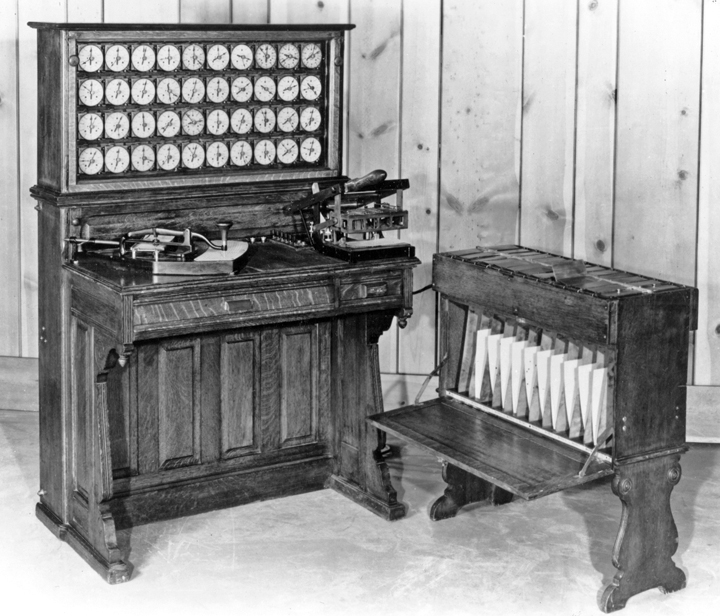
\includegraphics[height=5.3 cm]{hollerith.jpg}\hspace{1 cm}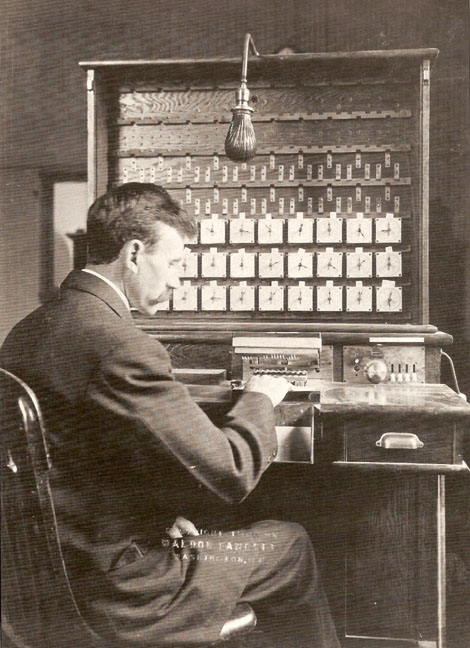
\includegraphics[height=5.3 cm]{1908_Hollerith_Machine.jpg}
\end{center}
\end{uncoverenv}
\end{frame}

\begin{frame}{Census records on punch cards, which filtered electrical contacts}
\vspace{0.17 cm}
\begin{columns}
\column{0.5\linewidth}
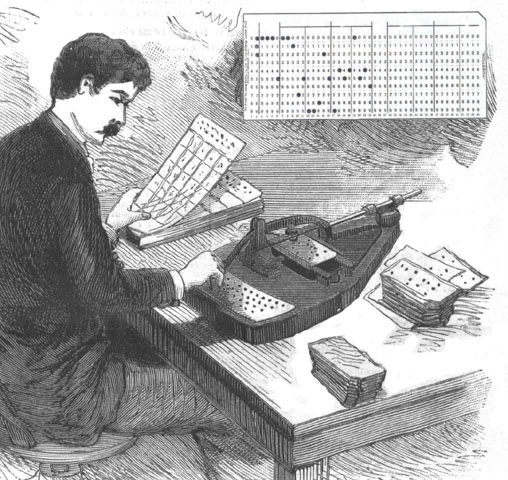
\includegraphics[width=\linewidth]{1890_Census_Hollerith_Pantograph_Punching_Machine_Sci_Amer.jpg}

\column{0.5\linewidth}
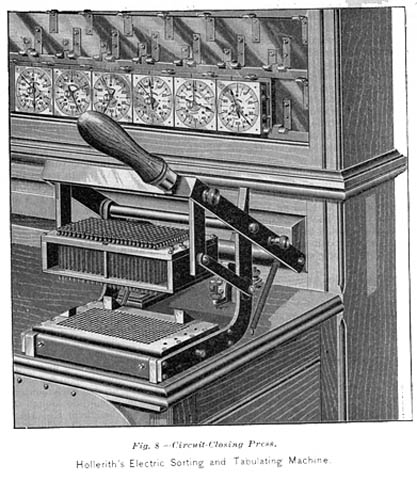
\includegraphics[width=\linewidth]{1890_Hollerith_Circuit-Closing_Press_OM.jpg}
\end{columns}
\end{frame}

\begin{frame}{Wired to a machine that opens a door for each matching pattern}
\vspace{0.25 cm}
\begin{center}
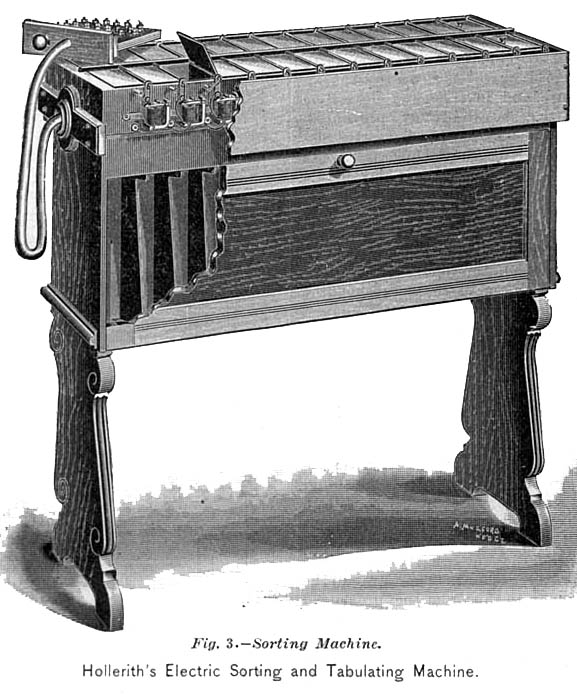
\includegraphics[width=0.45\linewidth]{1890_Hollerith_Sorting_Machine_OM.jpg}
\end{center}
\end{frame}

\begin{frame}{It was an SQL machine: 3 basic clauses of most SQL queries}
\vspace{0.25 cm}
\begin{center}
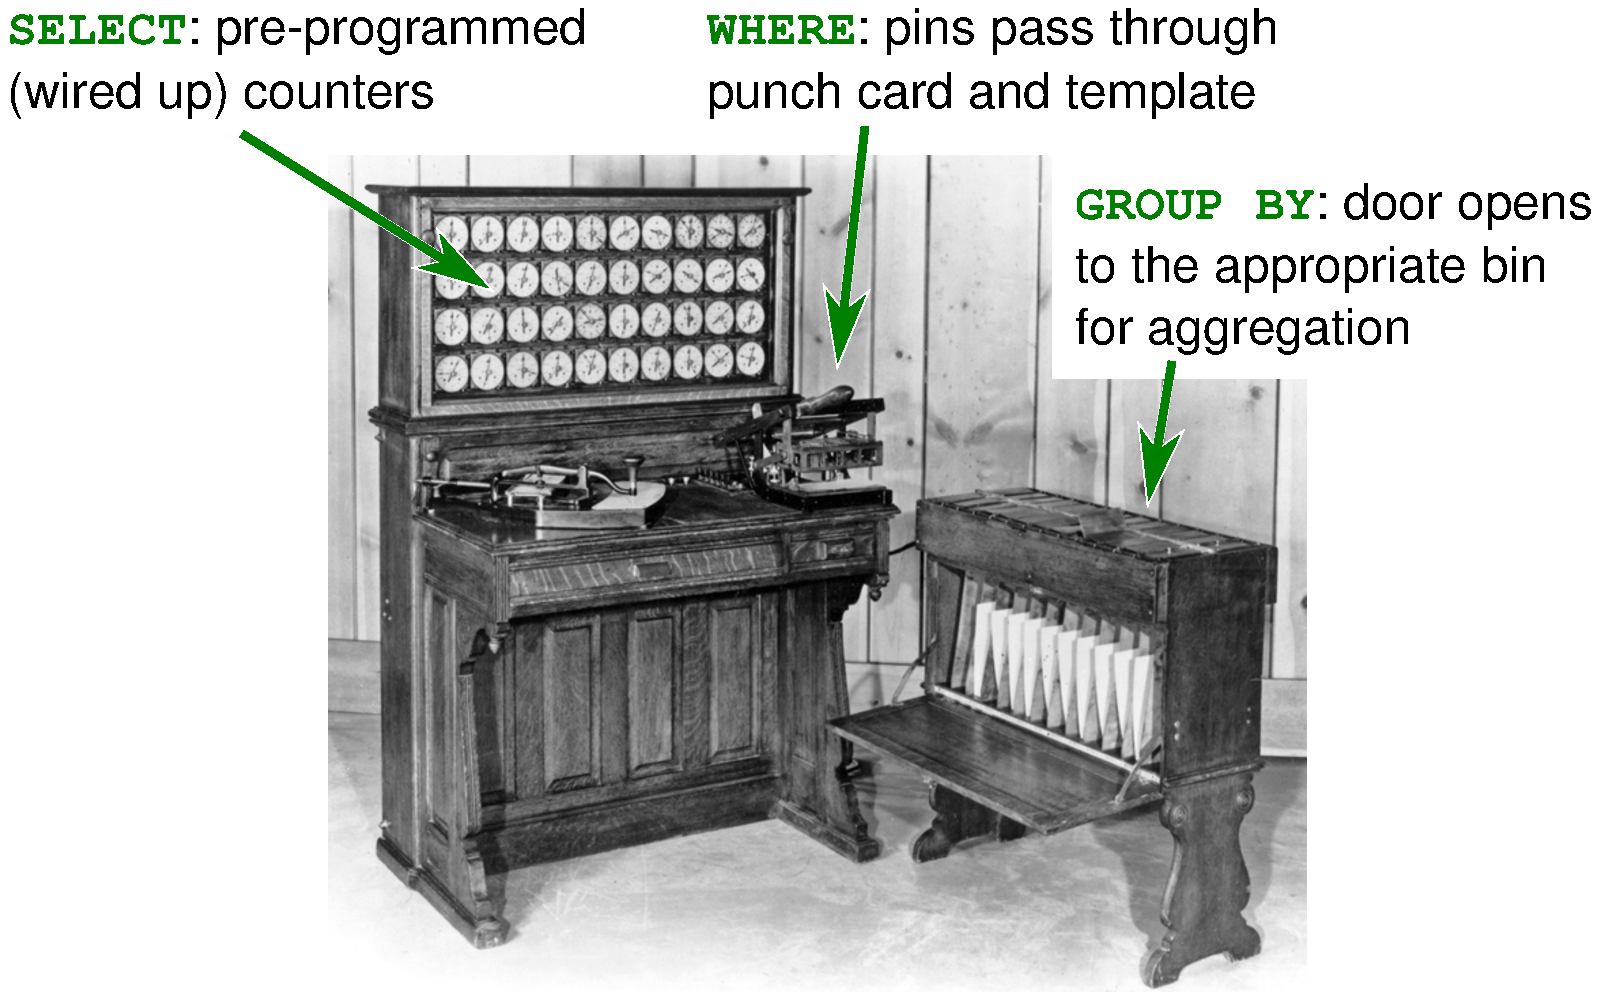
\includegraphics[width=0.75\linewidth]{hh-tabulator.pdf}
\end{center}

\mbox{ } \hfill \mintinline{sql}{SELECT name WHERE literate GROUP BY marital_status} \hfill \mbox{ }
\end{frame}

\begin{frame}{Origin of business computing}
\Large
\vspace{0.5 cm}
\begin{center}
Herman Hollerith founded a company selling these machines, which, after a series of mergers, became International Business Machines.
\end{center}

\small
\vspace{1 cm}
\textcolor{blue}{\url{https://www.officemuseum.com/data_processing_machines.htm}}

\vspace{0.25 cm}
\textcolor{blue}{\url{https://www.ibm.com/ibm/history/exhibits/builders/builders_hollerith.html}}
\end{frame}

\begin{frame}{Physics interest in computing came later}
\Large
\vspace{0.5 cm}
Nuclear/particle physics was a tabletop science before the Manhattan Project (nuclear bomb).

\normalsize
\vspace{0.75 cm}
\hfill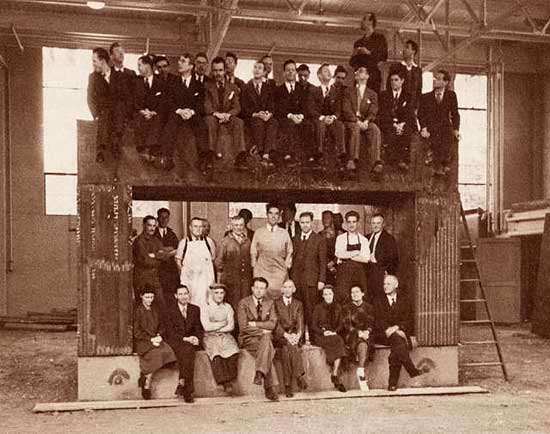
\includegraphics[height=2.5 cm]{bigsci-lblstaff.jpg}

\vspace{-3 cm}
\textcolor{darkblue}{\large Exceptions:}
\begin{itemize}
\item Ernest Lawrence's group at Berkeley (invented accelerators)

employed dozens---disparaged as ``Berkeleitis.''

\textcolor{blue}{\small\href{https://history.aip.org/history/exhibits/lawrence/epa.htm}{\tt https://history.aip.org/history/exhibits/\\lawrence/epa.htm}}

\item Cryogenics was big science in the early 20th century, but

that doesn't require much number-crunching.
\end{itemize}

\Large
\vspace{0.5 cm}
Physics and computing don't converge until the 1940's.
\end{frame}

\begin{frame}{Physicists got into computers when they became general-purpose}
\vspace{0.5 cm}

\begin{columns}
\column{0.3\linewidth}
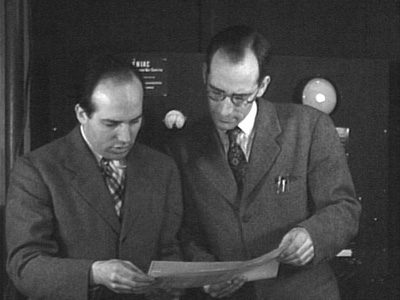
\includegraphics[width=\linewidth]{presper-and-mauchly.jpg}

\column{0.7\linewidth}
1944: John Mauchly (physicist) and J.\ Presper Eckert (electrical engineer) designed ENIAC to replace mechanical computers for ballistics.

\vspace{0.25 cm}
\uncover<2->{ENIAC was one of the first computers \textcolor{darkblue}{driven by machine code instructions}, stored as a program in memory.}
\end{columns}

\vspace{0.25 cm}
\begin{uncoverenv}<3->
\begin{columns}
\column{0.65\linewidth}
1945: John von Neumann learned of their work and suggested using it for nuclear simulations (H-bomb).

\vspace{0.25 cm}
\uncover<4->{His internal memo describing ENIAC's stored programs was leaked; now known as ``Von Neumann architecture.''}

\vspace{0.25 cm}
\uncover<5->{Los Alamos group led by Nicholas Metropolis, developed Monte Carlo techniques for physics problems.}
\column{0.35\linewidth}
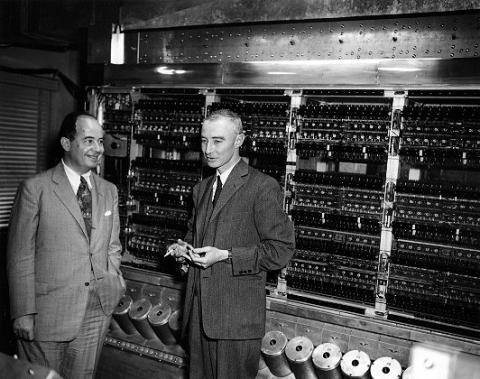
\includegraphics[width=\linewidth]{neumann_oppie.jpg}
\end{columns}
\end{uncoverenv}
\end{frame}

\begin{frame}{{\bf M}etropolis {\bf A}nd {\bf N}eumann {\bf I}nvent {\bf A}wful {\bf C}ontraption}
\small
\vspace{0.25 cm}

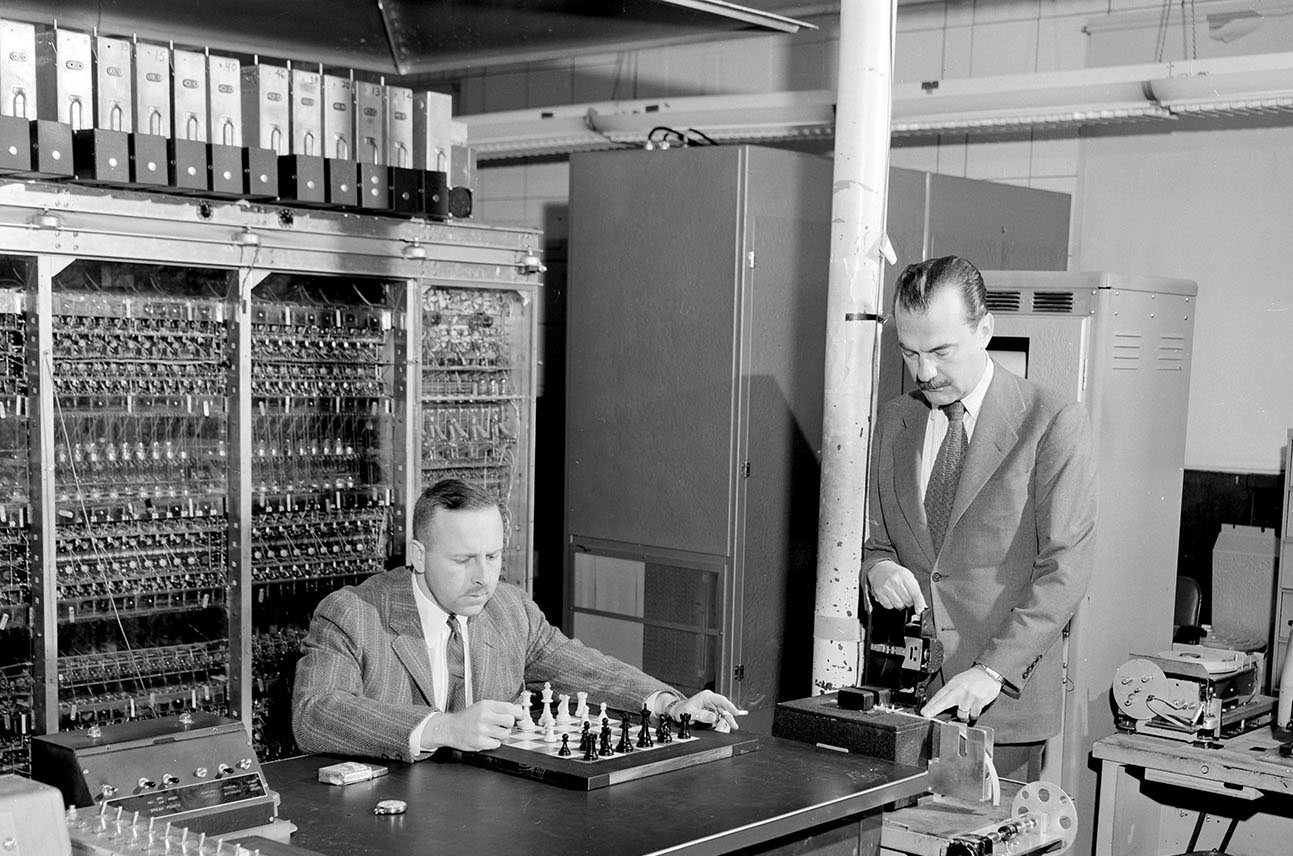
\includegraphics[height=5 cm]{metropolis.jpg}\hspace{0.1 cm}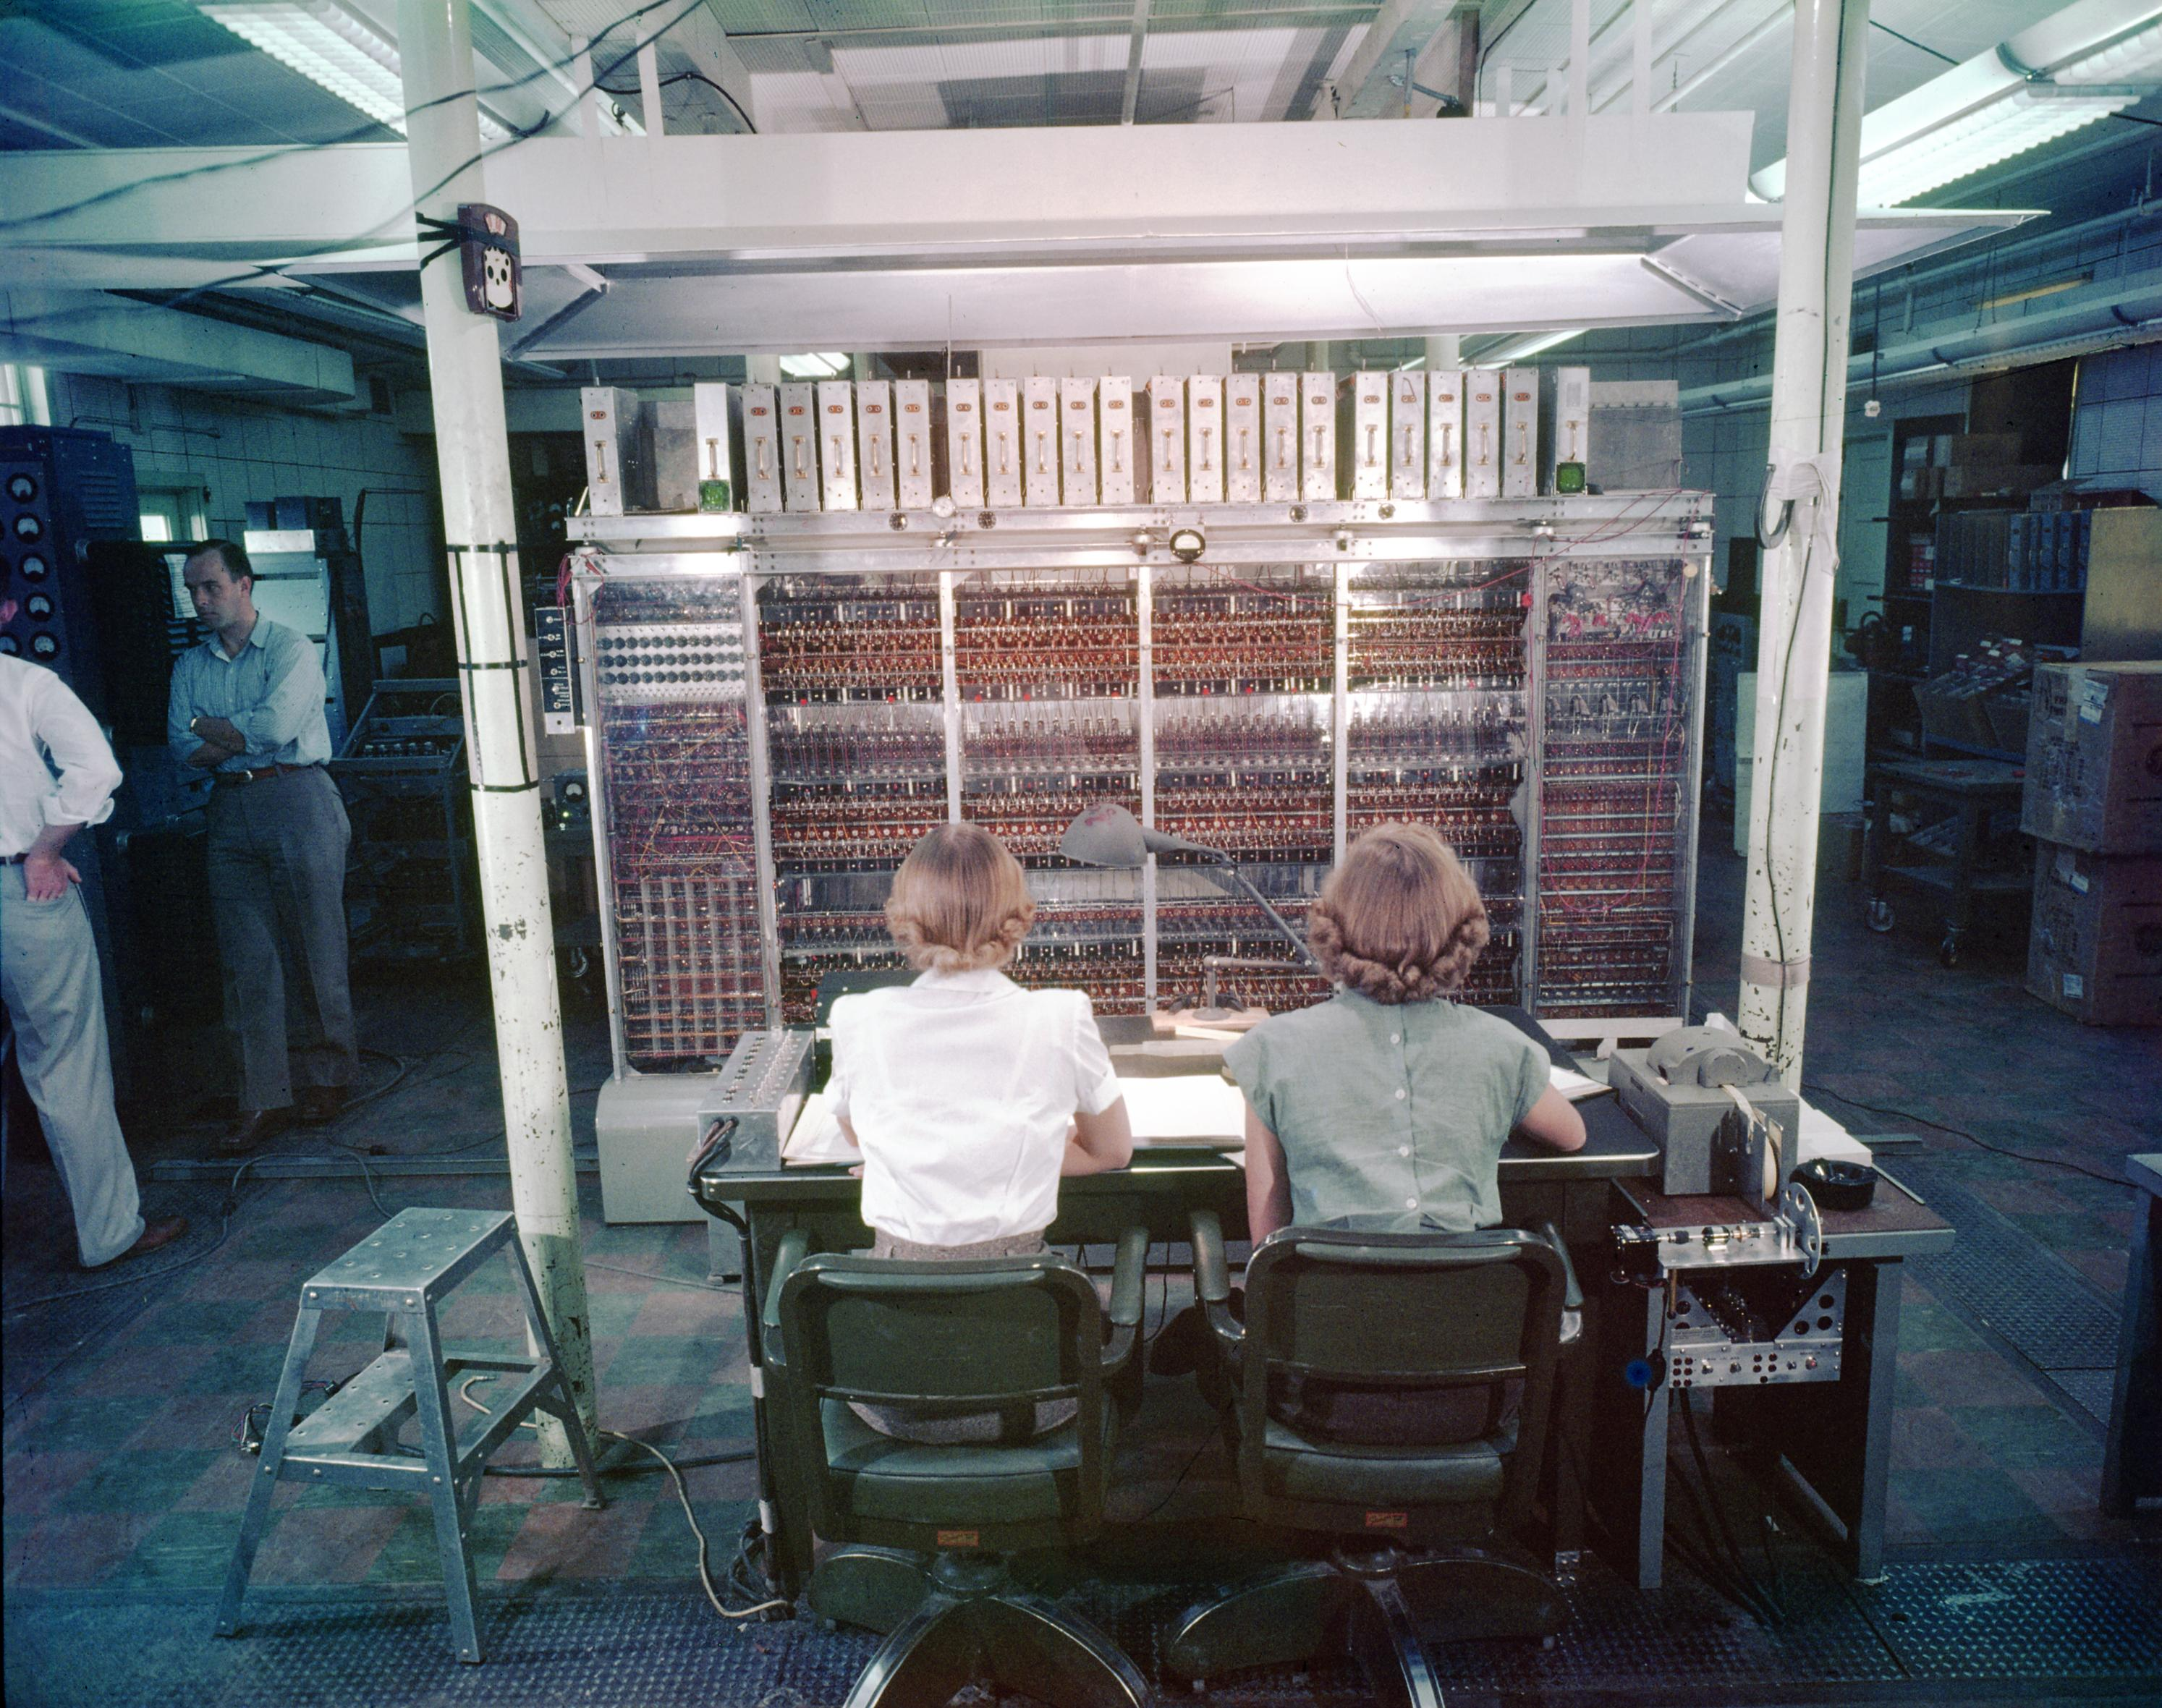
\includegraphics[height=5 cm]{1952-Maniac-1.jpg}

\vspace{0.25 cm}
\begin{columns}
\column{1.1\linewidth}
\textcolor{blue}{\url{https://www.atomicheritage.org/history/computing-and-manhattan-project}}

\vspace{0.1 cm}
\textcolor{blue}{\url{https://www.manhattanprojectvoices.org/oral-histories/nicholas-metropolis-interview}}

\vspace{0.1 cm}
\textcolor{blue}{\url{https://www.jstor.org/stable/20025423}}

\vspace{0.1 cm}
\textcolor{blue}{\url{https://books.google.com/books?id=qB819m2ibUQC}}
\end{columns}
\end{frame}

\begin{frame}{The actual programming was performed by these six women}
\begin{columns}[t]
\column{0.15\linewidth}
\begin{center}
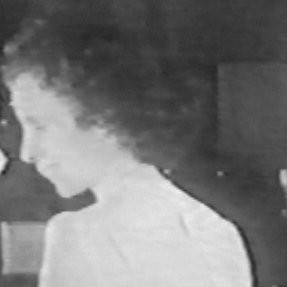
\includegraphics[width=\linewidth]{Kay-McNulty.jpg}

Kathleen McNulty
\end{center}

\column{0.15\linewidth}
\begin{center}
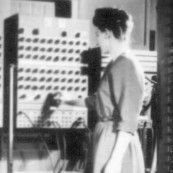
\includegraphics[width=\linewidth]{Fran-Bilas.jpg}

Frances Bilas
\end{center}

\column{0.15\linewidth}
\begin{center}
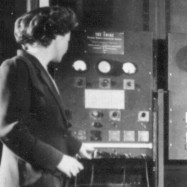
\includegraphics[width=\linewidth]{Betty-Jennings.jpg}

Betty Jean Jennings
\end{center}

\column{0.15\linewidth}
\begin{center}
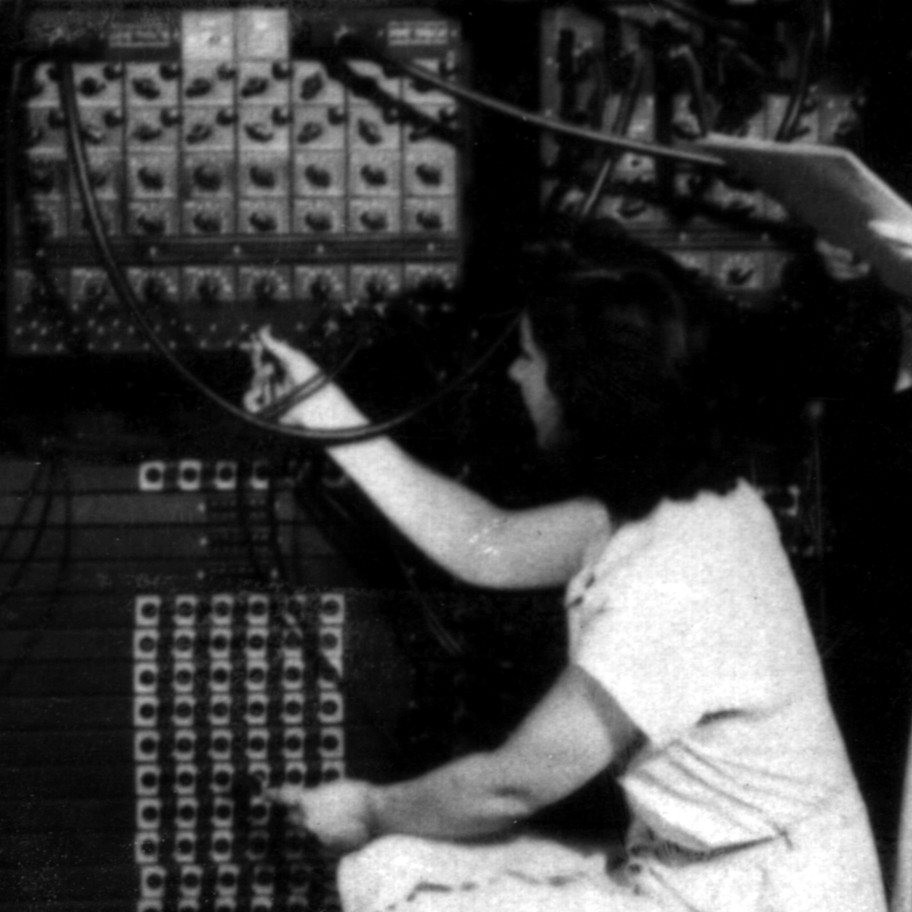
\includegraphics[width=\linewidth]{Ruth-Lichterman.jpg}

Ruth Lichterman
\end{center}

\column{0.15\linewidth}
\begin{center}
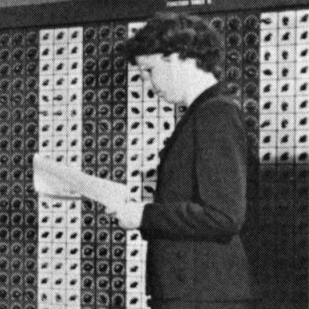
\includegraphics[width=\linewidth]{Betty-Snyder.jpg}

Elizabeth Snyder
\end{center}

\column{0.15\linewidth}
\begin{center}
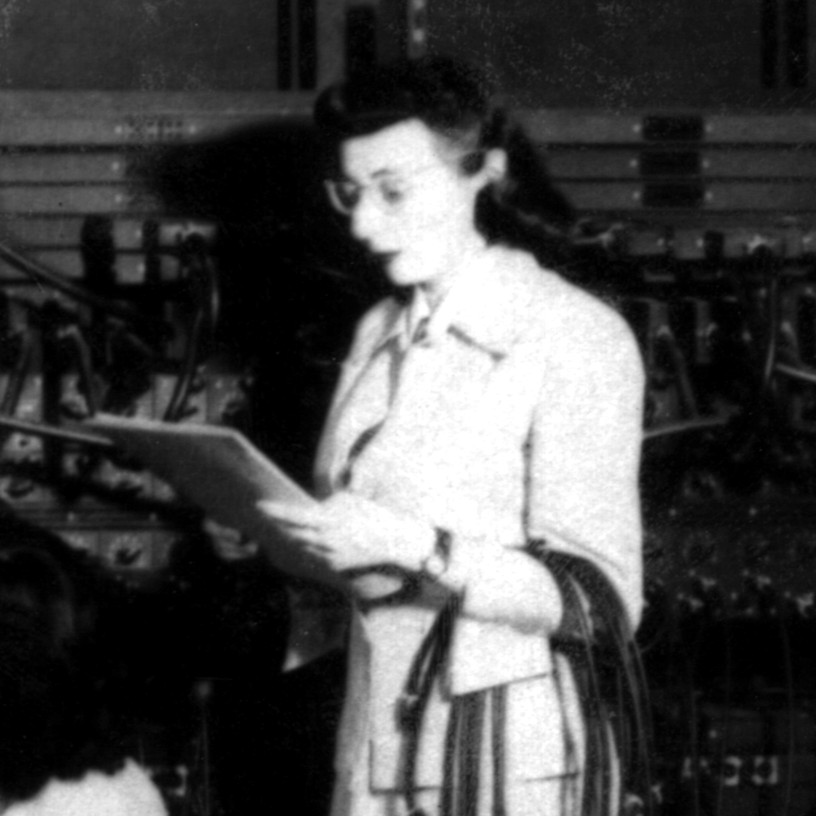
\includegraphics[width=\linewidth]{Marlyn-Meltzer.jpg}

Marlyn Wescoff
\end{center}
\end{columns}

\small
\vspace{1 cm}
\textcolor{blue}{\url{http://eniacprogrammers.org/eniac-programmers-project/}}

\vspace{0.5 cm}
\textcolor{blue}{\url{http://mentalfloss.com/article/53160/meet-refrigerator-ladies-who-programmed-eniac}}
\end{frame}





\end{document}
